\documentclass[12pt]{article}\usepackage[]{graphicx}\usepackage[]{color}
%% maxwidth is the original width if it is less than linewidth
%% otherwise use linewidth (to make sure the graphics do not exceed the margin)
\makeatletter
\def\maxwidth{ %
  \ifdim\Gin@nat@width>\linewidth
    \linewidth
  \else
    \Gin@nat@width
  \fi
}
\makeatother

\definecolor{fgcolor}{rgb}{0.345, 0.345, 0.345}
\newcommand{\hlnum}[1]{\textcolor[rgb]{0.686,0.059,0.569}{#1}}%
\newcommand{\hlstr}[1]{\textcolor[rgb]{0.192,0.494,0.8}{#1}}%
\newcommand{\hlcom}[1]{\textcolor[rgb]{0.678,0.584,0.686}{\textit{#1}}}%
\newcommand{\hlopt}[1]{\textcolor[rgb]{0,0,0}{#1}}%
\newcommand{\hlstd}[1]{\textcolor[rgb]{0.345,0.345,0.345}{#1}}%
\newcommand{\hlkwa}[1]{\textcolor[rgb]{0.161,0.373,0.58}{\textbf{#1}}}%
\newcommand{\hlkwb}[1]{\textcolor[rgb]{0.69,0.353,0.396}{#1}}%
\newcommand{\hlkwc}[1]{\textcolor[rgb]{0.333,0.667,0.333}{#1}}%
\newcommand{\hlkwd}[1]{\textcolor[rgb]{0.737,0.353,0.396}{\textbf{#1}}}%

\usepackage{framed}
\makeatletter
\newenvironment{kframe}{%
 \def\at@end@of@kframe{}%
 \ifinner\ifhmode%
  \def\at@end@of@kframe{\end{minipage}}%
  \begin{minipage}{\columnwidth}%
 \fi\fi%
 \def\FrameCommand##1{\hskip\@totalleftmargin \hskip-\fboxsep
 \colorbox{shadecolor}{##1}\hskip-\fboxsep
     % There is no \\@totalrightmargin, so:
     \hskip-\linewidth \hskip-\@totalleftmargin \hskip\columnwidth}%
 \MakeFramed {\advance\hsize-\width
   \@totalleftmargin\z@ \linewidth\hsize
   \@setminipage}}%
 {\par\unskip\endMakeFramed%
 \at@end@of@kframe}
\makeatother

\definecolor{shadecolor}{rgb}{.97, .97, .97}
\definecolor{messagecolor}{rgb}{0, 0, 0}
\definecolor{warningcolor}{rgb}{1, 0, 1}
\definecolor{errorcolor}{rgb}{1, 0, 0}
\newenvironment{knitrout}{}{} % an empty environment to be redefined in TeX

\usepackage{alltt}
% \usepackage{geometry}                % See geometry.pdf to learn the layout options. There are lots.
% \geometry{letterpaper}                   % ... or a4paper or a5paper or ... 
%\usepackage{graphicx}
\usepackage[font=small,skip=5pt]{caption}
\usepackage{subcaption}
\usepackage{afterpage}
\usepackage{amssymb}
\usepackage{natbib}
\usepackage{amsmath}
\usepackage{amsfonts}
% \usepackage{color}
\usepackage{multirow}
\usepackage{rotating}
\usepackage[dvipsnames,svgnames,table]{xcolor}
\usepackage{hyperref}
\graphicspath{{figure/}}
% \usepackage{endfloat} % Figures to the end of the document

\DeclareGraphicsRule{.tif}{png}{.png}{`convert #1 `dirname #1`/`basename #1 .tif`.png}
\usepackage[colorinlistoftodos]{todonotes}
%---------------------------------------------------
%                 Editing Commands
\newcommand{\done}[2][inline]{\todo[color=SpringGreen, #1]{#2}}  % for todos that have been seen and dealt with
\newcommand{\meh}[2][inline]{\todo[color=White, #1]{#2}}   % for todos that may no longer be relevant 
\newcommand{\comment}[2][inline]{\todo[color=SkyBlue, #1]{#2}} % for comments that may not be "to-do"s
%\newcommand{\mcomment}[1]{\todo[color=SkyBlue]{#1}} % for margin comments
\newcommand{\newtext}[1]{\todo[inline, color=White]{ \color{OliveGreen}{#1}}} % new text - not necessarily something to be done
\newcommand{\newdo}[1]{\todo[inline, color=Lime]{#1}} % new to do item
%
%---------------------------------------------------
%                 Placing Figures


%---------------------------------------------------
% Define new environment
\newtheorem{theorem}{Theorem}[section]
\newtheorem{algorithm}[theorem]{Algorithm}
%---------------------------------------------------

%\pdfminorversion=4
% NOTE: To produce blinded version, replace "0" with "1" below.
\newcommand{\blind}{0}

% DON'T change margins - should be 1 inch all around.
\addtolength{\oddsidemargin}{-.5in}%
\addtolength{\evensidemargin}{-.5in}%
\addtolength{\textwidth}{1in}%
\addtolength{\textheight}{1.3in}%
\addtolength{\topmargin}{-.8in}%
\IfFileExists{upquote.sty}{\usepackage{upquote}}{}
\begin{document}

%\bibliographystyle{natbib}

\def\spacingset#1{\renewcommand{\baselinestretch}%
{#1}\small\normalsize} \spacingset{1}


%%%%%%%%%%%%%%%%%%%%%%%%%%%%%%%%%%%%%%%%%%%%%%%%%%%%%%%%%%%%%%%%%%%%%%%%%%%%%%

\if0\blind
{
  \title{\bf Clusters beat Trend!? \\Testing feature hierarchy in statistical graphics}
  \author{Susan VanderPlas\thanks{
    The authors gratefully acknowledge funding from the National Science Foundation Grant \# DMS 1007697. All data collection has been conducted with approval from the Institutional Review Board IRB 10-347}\hspace{.2cm}\\
    Department of Statistics and Statistical Laboratory, Iowa State University\\
    and \\
    Heike Hofmann\\
    Department of Statistics and Statistical Laboratory, Iowa State University}
  \maketitle
} \fi

\if1\blind
{
  \bigskip
  \bigskip
  \bigskip
  \begin{center}
    {\LARGE\bf Clusters beat Trend!? \\Testing feature hierarchy in statistical graphics}
\end{center}
  \medskip
} \fi

\bigskip
\begin{abstract}
Graphics are very effective for communicating numerical information quickly and efficiently, but many of the design choices we make are based on subjective measures, such as personal taste or conventions of the discipline rather than objective criteria. We briefly introduce perceptual principles such as preattentive features and gestalt heuristics, and then discuss the design and results of a factorial experiment examining the effect of plot aesthetics such as color and trend lines on participants' assessment of ambiguous data displays. The quantitative and qualitative experimental results strongly suggest that plot aesthetics have a significant impact on the perception of important features in data displays. 
\end{abstract}

\noindent%
{\it Keywords:}  Visual inference, Lineup protocol, Preattentive Features, Saliency of Plot Aesthetics, User Study.
\vfill

\newpage
\spacingset{1.45} % DON'T change the spacing!

%\tableofcontents
\newpage
\section{Introduction and Background}
Limits on attention span, short term memory, and information storage mechanisms within the human brain make it difficult for us to process numerical information  in raw form effectively. 
(Well-designed) data displays are much better suited for this kind of communication, as  they serve as a form of external cognition \citep{zhang1997nature,scaife1996external}, ordering and visually summarizing data
and thereby invoking our higher-bandwidth visual system. 

One fantastic example of this phenomenon is the Hertzsprung-Russell (HR) diagram, which was described as ``one of the greatest observational syntheses in astronomy and astrophysics" because it allowed astronomers to clearly relate the absolute magnitude of a star to its' spectral classification; facilitating greater understanding of stellar evolution \citep{spence1993remarkable}. 
The data it displayed was previously available in several different tables; but when plotted within the same chart, information that was invisible in a tabular representation became immediately clear \citep{lewandowsky1989perception}. 
Graphical displays more efficiently utilize cognitive resources by reducing the burden of storing, ordering, and summarizing raw data; this frees bandwidth for higher levels of information synthesis, allowing observers to note outliers, understand relationships between variables, and form new hypotheses.

Graphical displays are powerful because they efficiently and effectively convey numerical information, but there exists  relatively sparse empirical information about how the human perceptual system processes these displays. Our understanding of the perception of statistical graphics is informed by general psychological and psychophysics research as well as more specific research into the perception of data displays \citep{cleveland:1984}. 

One relevant focus of psychological research is preattentive perception, that is, perception which occurs automatically in the first 200 ms of exposure to a visual stimulus \citep{treisman1985preattentive}. 

Research into {\bf preattentive perception} provides us with some information about the temporal hierarchy of graphical feature processing. Color, line orientation, and shape are processed preattentively; that is, within 200 ms, it is possible to identify a single target in a field of distractors, if the target differs with respect to color or shape \citep{goldstein2009encyclopedia}. 
Research by \citet{healey1999large} extends this work, demonstrating that certain features of three-dimensional data displays are also processed preattentively. However, neither target identification nor three-dimensional data processing always translate into faster or more accurate inference about the data displayed, particularly when participants have to integrate several preattentive features to understand the data. 

{\bf Feature detection} at the attentive stage of perception has also been examined in the context of statistical graphics; researchers have evaluated the perceptual implications of utilizing color, fill, shapes, and letters to denote categorical or stratified data in scatterplots. \citet{cleveland:1984} ranked the optimality of these plot aesthetics based on response accuracy, preferring colors, amount of fill, shapes, and finally letters to indicate category membership. \citet{lewandowsky1989discriminating} examined both accuracy and response time, finding that color is faster and more accurately perceived (except by individuals with color deficiency). Shape, fill, and discriminable letters (letters which do not share visual features, such as HQX) were identified as less accurate than color, while confusable letters (such as HEF) result in significantly decreased accuracy. 

{\bf Gestalt psychology} is another area of psychological research, that examines perception as a holistic experience, establishing and evaluating mental heuristics used to transform visual stimuli into useful, coherent information. 
Gestalt rules of perception can be easily applied to statistical graphics, as they describe the way we organize visual input, focusing on the holistic experience rather than the individual perceptual features. 

For example, rather than perceiving four legs, a tail, two eyes, two ears, and a nose, we perceive a dog. This is due to certain perceptual heuristics, which provide a ``top-down" method of understanding visual stimuli by taking into account past experience. 

The rules of perceptual organization relevant to graphical perception in this experiment are:
\begin{itemize}
\item \textbf{Proximity}: two elements which are close together are more likely to belong to a single unit.
\item \textbf{Similarity}: the more of the same or similar aesthetics two elements share two elements are, the more likely they belong to a single unit. 
\item \textbf{Good continuation}: two elements which blend together smoothly likely belong to one unit.
\item \textbf{Common region}: elements contained within a common region likely belong together. 
\end{itemize}
A complete list of the rules of perceptual grouping can be found in \citet{goldstein2009encyclopedia}.

\begin{figure}\centering
\begin{knitrout}
\definecolor{shadecolor}{rgb}{0.969, 0.969, 0.969}\color{fgcolor}

{\centering \includegraphics[width=0.32\linewidth]{figure/gestalt1-1} 
\includegraphics[width=0.32\linewidth]{figure/gestalt1-2} 
\includegraphics[width=0.32\linewidth]{figure/gestalt1-3} 

}



\end{knitrout}
\caption[Gestalt principles applied to statistical plots]{\label{fig:gestalt} \emph{Proximity} renders the fifty points of the first scatterplot as two distinct (and equal-sized) groups. Shapes and colors create three groups of points in the middle scatterplot by invoking the Gestalt principle of \emph{Similarity}. \emph{Good Continuation} renders the points in the scatterplot on the right hand side into two groups of points on curves: one a straight line with an upward slope, the other a curve that initially decreases and at the end of the range shows an uptick.}
\end{figure}

The plots in Figure~\ref{fig:gestalt} demonstrate several of the gestalt principles which combine to order our perceptual experience from the top down. These laws help to order our perception of charts as well: points which are colored or shaped the same are perceived as belonging to a group (similarity), points within a bounding interval or ellipse are perceived as belonging to the same group (common region), and regression lines with confidence intervals are perceived as single units (continuity and common region). 

The processing of visual stimuli utilizes low-level feature detection, which occurs automatically in the preattentive perceptual phase, and higher-level mental heuristics which are informed by experience. Both types of mental processes utilize physical location, color, and shape  to organize perceptual stimuli and direct attention to graphical features which stand out. 

Research on preattentive perception is important because features that are perceived preattentively require less mental effort to process from raw visual stimuli than non-preattentive features. Top-down gestalt heuristics are subsequently applied to the categorized features in order to make sense of the visual scene once the attentive stage of perception is reached. 


This paper describes the design and the results of a user study exploring the hierarchy of gestalt principles in the perception of statistical graphics. We utilize information from previous studies~\citep{heer:2014, robinson:03, healey1996high} concerning the hierarchy of preattentive feature perception in order to maximize the effect of preattentive feature differences. 


Statistical graphics can be difficult to examine experimentally; qualitative studies rely on descriptions of the plot by participants who may not be able to articulate their observations precisely, while quantitative studies may only be able to examine whether the viewer can accurately read numerical information from the chart, instead of exploring the overall utility of the data display holistically. Here, we are describing the setup and results of a study using statistical lineup methodology to provide quantitative and qualitative information.

\paragraph{Statistical lineups} are an important experimental tool for quantifying the significance of a finding in a graphical display. 
Lineups fuse commonly used psychological tests (target identification, visual search) \citep{visualreasoning} with statistical hypothesis tests, thereby enabling formal experimental evaluation of statistical graphics. 

Lineups are an experimental tool designed to serve as a visually conducted hypothesis test, separating significant effects from those that would be expected under a null hypothesis \citep{buja2009statistical, majumder2013validation,hofmann2012graphical, wickham2010graphical}. 
A statistical lineup consists of (usually) 20 sub-plots, arranged in a grid (examples are shown in Figure~\ref{fig:plotExamples}). 
Of these plots, one plot is the ``target plot'', generated from either real data or an alternate model (equivalent to $H_A$ in hypothesis testing); the other 19 plots are generated either using bootstrap samples of the real data or by generating ``true null" plots from the null distribution $H_0$. 
If a participant can identify the target plot from the field of distractors, this counts as evidence against the null hypothesis. 
Based on the number of evaluations and the number of target identifications, significance of a finding is then determined in the same sense as for a conventional hypothesis test. 
Apart from the hypothesis testing construct, the use of statistical lineups to test statistical graphics conforms nicely to psychological testing constructs such as visual search \citep{demita1981validity,treisman1980feature}, where a single target is embedded in a field of distractors and response time, accuracy, or both are used to measure the complexity of the underlying psychological processes leading to identification. 

In this paper we {\bf modify the lineup protocol} by introducing a second target to each lineup. 
The two targets represent two different, competing signals; an observer's choice then demonstrates empirically which signal is more salient. 
If both targets exhibit similar signal, observers may identify both targets, removing any forced-choice scenario which might skew results in a study. 

%By tracking the proportion of observers choosing either target plot (a measure of overall lineup difficulty) as well as which proportion of observers choose one target over the other target, we can determine the relative strength of the two competing signals amid a field of distractors. 
%At this level, signal strength is determined by the experimental data and the generating model; we are measuring the ``power" (in a statistical sense) of the human perceptual system, rather than raw numerical signal. 

Using this testing framework, we  apply different aesthetics, such as color and shape, as well as plot objects which display statistical calculations, such as trend lines and bounding ellipses. 
These additional plot layers, discussed in more detail in the next section, are designed to emphasize one of the two competing targets and affect the overall visual signal of the target plot relative to the null plots. 
We expect that in a situation similar to the third plot of Figure~\ref{fig:gestalt}, the addition of two trend lines would emphasize the ``good continuation" of points in the plot, producing a stronger visual signal, even though the underlying data has not changed. 
Similarly, the grouping effect in the first plot in the figure should be enhanced if the points in each group are colored differently, as this adds similarity to the proximity heuristic. 
In plots that are ambiguous, containing some clustering of points as well as a linear relationship between $x$ and $y$, additional aesthetic cues may ``tip the balance" in favor of recognizing one type of signal over the other.

The study in this paper is designed to inform our understanding of the perceptual implications of these additional aesthetics, in order to provide guidelines for the creation of data displays which provide visual cues consistent with gestalt heuristics and preattentive perceptual preferences. 

The next section discusses the particulars of the experimental design, including the data generation model, plot aesthetics, selection of color and shape palettes, and other important considerations. 
Experimental results are presented in section \ref{sec:Results}, and implications and conclusions are discussed in section \ref{sec:Conclusion}. 

\section{Experimental Setup and Design} \label{sec:ExperimentalDesign}
In this section, we discuss the models generating data for the two types of signal plots and the null plots, the selection of plot aesthetic combinations and aesthetic values, and the design and execution of the experiment.

\subsection{Data Generation}
Conventional lineups require a single ``target" data set and a method for generating null plots. 
When utilizing real data for target plots, null plots are often generated through permutations.

Here, it is possible to generate true null plots from a null model that do not depend on the data used in the target plot. 
This experiment measures two competing gestalt heuristics, proximity and good continuation, using two data-generating models. 
Both models provide data in the same range of values in $X$ and $Y$;  $M_C$ generates data  with $K$ clusters, while $M_T$ generates data with a positive linear relationship between $X$ and $Y$. 
Null datasets are created using a mixture model $M_0$ which combines $M_C$ and $M_T$. 
In order to facilitate mixing these two models, controls on cluster centers generated by $M_C$ ensure that $X$ and $Y$ have a positive linear relationship with a correlation $\rho \in (0.25, 0.75)$, similar to the linear relationship between datasets generated by $M_0$. 

These constraints provide some assurance that participants who select a plot with data generated from $M_T$ are doing so because of visual cues indicating a linear trend (rather than a lack of clustering compared to plots with data generated from $M_0$), and participants who select a plot with data generated from $M_C$ are doing so because of visual cues indicating clustering, rather than a lack of a linear relationship relative to plots with data generated from $M_0$. 

\subsubsection{Regression Model \texorpdfstring{$M_T$}{Mt}}
This model has the parameter $\sigma_T$ to reflect the amount of scatter around the trend line. It generates $N$ points $(x_i, y_i), i=1, ..., N$ where $x$ and $y$ have a positive linear relationship. The data generation mechanism is as follows: 

\begin{algorithm}\hfill\newline
  Input Parameters: sample size $N$, $\sigma_T$ standard deviation around the line \\
  Output: $N$ points, in form of vectors $x$ and $y$.
  \begin{enumerate}
    \item Generate $\tilde{x}_i$, $i=1, ..., N$, as a sequence of evenly spaced points in $[-1, 1]$.\\
    This step ensures that the full range in $x$ is used, which in turn keeps the ratio of $x$ to $y$ range constant.
    \item Jitter $\tilde{x}_i$ by adding small uniformly distributed perturbations to each of the values: $x_i = \tilde{x}_i + \eta_i$, where $\eta_i \sim \text{Unif}(-z, z)$, $z = \frac{2}{5(N-1)}$.
    \item Generate $y_i$ as a linear regressand of $x_i$: $y_i = x_i + e_i$, $e_i \sim N(0, \sigma^2_T)$.
    \item Center and scale $x_i$, $y_i$.
  \end{enumerate}
\end{algorithm}

We compute the coefficient of determination for all of the plots to assess the amount of linearity in each panel, computed as 
\begin{equation}\label{eq:linearMeasure}
R^2 = 1 - \frac{RSS}{TSS},
\end{equation}
where TSS is the total sum of squares, $TSS = \sum_{i=1}^N \left(y_i - \bar{y}\right)^2$ and $RSS = \sum_{i=1}^N e_i^2$, the residual sum of squares.
The expected value of the coefficient of determination $E\left[R^2\right]$ in this scenario is 
\[
E\left[R^2\right] =  \frac{1}{1 + 3\sigma^2_T},
\]
because
$E[RSS] = N\sigma^2_T$ and $E[TSS] = \sum_{i=1}^N E\left[y_i^2\right]$  (as $E[Y] = 0$), where 
$$
E\left[y_i^2\right] = E\left[x_i^2 + e_i^2 + 2 x_ie_i\right] = \frac{1}{3} + \sigma^2_T. 
$$
The use of $R^2$ to assess the strength of the linear relationship (rather than the correlation) is indicated because human perception of correlation strength more closely aligns with $R^2$ \citep{bobko1979perception,lewandowsky1989perception}. 

\begin{figure}[ht]
\begin{knitrout}
\definecolor{shadecolor}{rgb}{0.969, 0.969, 0.969}\color{fgcolor}

{\centering \includegraphics[width=\linewidth]{figure/trends-1} 

}



\end{knitrout}
\caption[Parameters affecting $M_T$]{\label{fig:trends} Set of scatterplots showing one draw each from the trend model $M_T$ for parameter values of  $\sigma_T \in \{0.1, 0.2, 0.3, 0.4\}$.}
\end{figure}

\subsubsection{Cluster Model \texorpdfstring{$M_C$}{Mc}} 
We begin by generating $K$ cluster centers on a $K \times K$ grid, then we generate points around selected cluster centers. 
\begin{algorithm}\hfill\newline
  Input Parameters:  $N$ points, $K$ clusters, $\sigma_C$ cluster standard deviation \\
  Output: $N$ points, in form of vectors $x$ and $y$. 
  \begin{enumerate}
    \item Generate cluster centers $(c^x_{i}, c^y_{i})$ for each of the $K$ clusters, $i=1, ..., K$:
      \begin{enumerate}
        \item in form of two vectors $c^{x}$ and $c^y$ of permutations of $\{1, ..., K\}$, such that
        \item the correlation between cluster centers \text{cor}$(c^{x}, c^{y})$ falls into a range of $[.25, .75]$.
      \end{enumerate}
      \item Center and standardize cluster centers $(c^x, c^y)$:  
      \[
        \tilde{c}^x_{i} = \frac{c^x_{i} - \bar{c}}{s_c} \ \ \text{ and } \ \ \tilde{c}^y_{i} = \frac{c^y_{i} - \bar{c}}{s_c},
      \]
      where $\overline{c} = (K+1)/2$ and $s_c^2 = \frac{K(K+1)}{12}$ for all $i = 1, ..., K$.
    \item For the $K$ clusters, we want to have nearly equal sized groups, but allow some variability. Cluster sizes  $g = (g_1, ..., g_K)$ with $N = \sum_{i=1}^K g_i$, for clusters $1, ..., K$ are therefore determined as a draw from a multinomial distribution: 
    \[
    g \sim \text{Multinomial }(K, p) \text{ where } p = \tilde{p}/\sum_{i=1}^K \tilde{p}_i, \text{ for } \tilde{p} \sim N \left(\frac{1}{K}, \frac{1}{2 K^2} \right).
    \]
     
    \item Generate points around cluster centers by adding small normal perturbations: 
      \begin{eqnarray*}
        x_i &=& \tilde{c}^x_{g_i} + e^x_i, \text{ where } e^x_i \sim N(0, \sigma^2_C),\\
        y_i &=& \tilde{c}^y_{g_i} + e^y_i, \text{ where } e^y_i \sim N(0, \sigma^2_C).
      \end{eqnarray*}
    \item Center and scale $x_i$, $y_i$.
  \end{enumerate}
\end{algorithm} 

\begin{figure}[bht]
\begin{knitrout}
\definecolor{shadecolor}{rgb}{0.969, 0.969, 0.969}\color{fgcolor}

{\centering \includegraphics[width=\linewidth]{figure/cluster-1} 

}



\end{knitrout}
\caption[Parameters affecting $M_C$]{\label{fig:clusters} 
Scatterplots of clustering output for different inner cluster spread $\sigma_C$  (left to right) and different number of clusters $K$ (top and bottom), generated using the same random seed at each parameter setting. 
The colors and shapes shown are those used in the lineups for $K=3$ and $K=5$.}
\end{figure}
As a measure of cluster cohesion we use a coefficient to assess the amount of variability within each cluster, compared to total variability. 
Note that for the purpose of clustering, variability is measured as the variability in both $x$ and $y$ from a common mean, i.e.\ we implicitly assume that the values in $x$ and $y$ are on the same scale. 
This ensures that $\sigma_C$is a scaling parameter that regulates the amount of cluster cohesion (see Figure~\ref{fig:clusters}).  

For two numeric variables $x$ and $y$ and grouping variable $g$ with $g_i \in \{1, ..., K\}, i = 1, ..., n$, we compute the  {\it cluster index} $C^2$ as follows: 
let $j(i)$ be the function that maps index $i = 1, ..., n$ to one of the clusters $1, ..., K$ given by the grouping variable $g$. 
Then for each  level of $g$, we find  a cluster center as $\bar{x}_{j(i)}$ and  $\bar{y}_{j(i)}$, and we determine the strength of the clustering by comparing the within cluster variability with the overall variability: 

\begin{eqnarray}\label{eq:clusterMeasure}
C^2 &=& 1 - \frac{CSS}{TSS},\\
\nonumber CSS &=& \sum_{i=1}^n \left(x_{j(i)} - \overline{x}_{j(i)}\right)^2 + \left(y_{j(i)} - \overline{y}_{j(i)} \right)^2, \\
\nonumber TSS &=& \sum_{i=1}^n \left(x_i - \bar{x}\right)^2 + \left(y_i - \bar{y}\right)^2.
\end{eqnarray}

The cluster index $C^2$, which is approximately inversely linear in $\sigma_C^2$, measures the actual amount of clustering in the generated data.



\subsubsection{Null Model \texorpdfstring{$M_0$}{M0}}
The generative model for null data is a mixture model $M_0$ that draws $n_c \sim \text{Binomial}(N, \lambda)$ observations from the cluster model, and $n_T = N - n_c$ from the regression model $M_T$. 
Observations are assigned to specific clusters using hierarchical clustering, which creates groups consistent with any structure present in the generated data. 
This provides a plausible grouping for use in aesthetic and statistics requiring categorical data (color, shape, bounding ellipses). 

\begin{figure}[hbt]
\begin{knitrout}
\definecolor{shadecolor}{rgb}{0.969, 0.969, 0.969}\color{fgcolor}

{\centering \includegraphics[width=.9\linewidth]{figure/lambda-1} 

}



\end{knitrout}
\caption[Mixing parameter for null model $M_0$]{\label{fig:lambda} Scatterplots of data generated from $M_0$ using different values of $\lambda$, generated using the same random seed at each $\lambda$ value.}
\end{figure}

Null data in this experiment is generated using $\lambda = 0.5$, that is, each point in a null data set is equally likely to have been generated from $M_C$ and $M_T$ to ensure maximal distance of the null plots from either target. 

\subsubsection{Parameters used in Data Generation}
Models $M_C$, $M_T$, and $M_0$ provide the foundation for this experiment; by manipulating cluster standard deviation $\sigma_C$ and regression standard deviation $\sigma_T$ for varying numbers of clusters $K=3, 5$, we  systematically control the statistical signal present in the target plots and generate corresponding null plots that are mixtures of the two distributions. 
For each parameter set $\{K, N, \sigma_C, \sigma_T\}$, as described in Table~\ref{tab:parameters}, we  generate a lineup dataset consisting of one set drawn from $M_C$, one set drawn from $M_T$, and 18 sets drawn from $M_0$. 

\begin{table}[hbtp]
  \rowcolors{2}{gray!25}{white}
\begin{center}
\begin{tabular}{lll}
\bf Parameter & \bf Description & \bf Choices\\\hline
$K$ & \# Clusters &  \begin{tabular}{l}3, 5 \end{tabular} \\
$N$ & \# Points &  \begin{tabular}{l}$15\cdot K$\end{tabular} \\
$\sigma_T$ & Scatter around trend line &   \begin{tabular}{l}.15, .25, .35  \end{tabular}\\
$\sigma_C$ & Scatter around cluster centers & \begin{tabular}{ll} .25, .30, .35 ($K=3$)\\ .20, .25, .30 ($K=5$) \end{tabular}
\\\hline
\end{tabular}
\end{center}
\caption{Parameter settings for generation of lineup datasets. \label{tab:parameters}}
\end{table}

The parameter values were chosen in an approach similar to that taken in \citet{niladri:2014}: for each combination of $\sigma_T\in\{0.2, 0.25, ..., 0.5\}$, $\sigma_C\in\{0.1, 0.15, ..., 0.4\}$, and $K\in\{3,5\}$ we simulated 1000 lineup datasets. 
Then trend and cluster strength indices, $R^2$ and $C^2$, were computed  for the simulated target plots, and compared to the most extreme value for each of the 18 null plots of the same lineup data.

The resulting distributions allow us to objectively assess the difficulty of detecting the target datasets computationally (without relying on human perception) within the full parameter space. 
That is, a target plot with $R^2=0.95$ is very easy to identify when surrounded by null plots with $R^2=0.5$, while null plots with $R^2=0.9$ make the target plot more difficult to identify. 

Figure~\ref{fig:targetsignal-0} shows  densities of each measure computed from the  maximum of 18 null plots compared to the measure in the signal plot for one combination of parameters.
There is some overlap in the distribution of $R^2$ for the null plots compared to the target plot displaying data drawn from $M_T$. 
As a result, the distribution of the cluster statistic values are more easily separated from the null data sets than the distribution of the line statistic, e.g. $\sigma_C = 0.20$ is producing cluster target data sets that are a bit easier to identify numerically than trend targets with a parameter value of $\sigma_T = 0.25$.

\begin{figure}[ht]
\centering
\begin{knitrout}
\definecolor{shadecolor}{rgb}{0.969, 0.969, 0.969}\color{fgcolor}

{\centering \includegraphics[width=\maxwidth]{figure/null-distribution-1-1} 

}



\end{knitrout}
\caption[Simulation-based test statistic density for null and target plots]{
\label{fig:targetsignal-0}
Density of test statistics measuring trend strength and cluster strength for target distributions and null plots based on 1,000 draws of lineup data with $\sigma_T= 0.25, \sigma_C=0.20$ and $K=3$.
}
\end{figure}

Graphical summaries of simulation results for a range of values for $\sigma_C$ and $\sigma_T$ are provided in appendix \ref{app:parametersimulation}. 
Using information from the simulation, we identified values and generate lineup data sets for each  $\sigma_T$ and $\sigma_C$ (as shown in Table~\ref{tab:parameters}) corresponding to ``easy", ``medium" and ``hard" numerical comparisons between corresponding target data sets and null data sets. 
It is important to note that the numerical measures we have described in equations~\eqref{eq:linearMeasure} and~\eqref{eq:clusterMeasure} only provide information on the numerical discriminability of the target datasets from the null datasets; the simulation cannot provide us with exact information on the perceptual discriminability.
It has been established that human perception of scatterplots does not replicate statistical measures exactly \citep{bobko1979perception, mosteller1981eye, lewandowsky1989perception}.

Each of the generated datasets is then plotted as a lineup using aesthetics, which emphasize clusters and/or linear relationships, to experimentally determine how these aesthetics change a participant's preference and ability to identify each target plot. 
The next section describes the aesthetic combinations and their anticipated effect on participant responses. 

\subsection{Lineup Rendering}
\subsubsection{Plot Aesthetics}
Gestalt perceptual theory suggests that perceptual features such as shape, color, trend lines, and boundary regions modify the perception of ambiguous graphs, emphasizing clustering in the data (in the case of shape, color, and bounding ellipses) or linear relationships (in the case of trend lines and prediction intervals), as demonstrated in Figure~\ref{fig:gestalt}. 
For each dataset we examine the effect of plot aesthetics (color, shape) and statistical layers (trend line, boundary ellipses, prediction intervals) shown in Table~\ref{tab:plotaesthetics}  on target identification.
Examples of these plot aesthetics are shown in Figure~\ref{fig:plotExamples}.

\begin{table}[hbtp]
\centering
\scalebox{0.8}{
\begin{tabular}{ccccc}
\begin{tabular}{c} \phantom{.}\\ \phantom{.} \end{tabular} && \multicolumn{3}{c}{\cellcolor{gray!25} Line Emphasis} \\
& Strength & 0 & 1 & 2 \\
\cellcolor{gray!25}\begin{tabular}{c} \phantom{.}\\ \phantom{.} \end{tabular} & 0 &  \cellcolor{gray!5} None &  \cellcolor{gray!15} Line &  \cellcolor{gray!25} Line + Prediction \\
\cellcolor{gray!25}\begin{tabular}{c} \\ Cluster \end{tabular} & 1 &  \cellcolor{gray!15}\begin{tabular}{c}Color\\ Shape\end{tabular} & \cellcolor{gray!5} Color + Line \\
\cellcolor{gray!25}\begin{tabular}{c}  Emphasis\\ \phantom{.} \end{tabular} & 2 & \cellcolor{gray!25}\begin{tabular}{c} Color + Shape\\ Color + Ellipse \end{tabular} && \cellcolor{gray!5}\begin{tabular}{c} Color + Ellipse +\\
Line + Prediction \end{tabular}\\
\cellcolor{gray!25}\begin{tabular}{c} \phantom{.}\\ \phantom{.} \end{tabular} & 3 & \cellcolor{gray!35} Color + Shape + Ellipse 
\end{tabular}}
\caption[Aesthetics affecting perception of statistical plots]{Plot aesthetics and statistical layers which impact perception of statistical plots, according to gestalt theory. \label{tab:plotaesthetics}}
\end{table}

\begin{figure}[ht]
\centering
\begin{subfigure}[t]{0.25\linewidth}
  \caption{Plain}\vspace{-0.15in}
  \includegraphics[width=\linewidth]{figure/samplepics-1}
\end{subfigure}
\begin{subfigure}[t]{0.25\linewidth}
  \caption{Color}\vspace{-0.15in}
  \includegraphics[width=\linewidth]{figure/samplepics-2}
\end{subfigure}
\begin{subfigure}[t]{0.25\linewidth}
  \caption{Shape}\vspace{-0.15in}
  \includegraphics[width=\linewidth]{figure/samplepics-3}
\end{subfigure}
\begin{subfigure}[t]{0.25\linewidth}
  \caption{Shape + Color}\vspace{-0.15in}
  \includegraphics[width=\linewidth]{figure/samplepics-4}
\end{subfigure}
\begin{subfigure}[t]{0.25\linewidth}
  \caption{Color + Ellipse}\vspace{-0.15in}
  \includegraphics[width=\linewidth]{figure/samplepics-5}
\end{subfigure}
\begin{subfigure}[t]{0.25\linewidth}
  \caption{Shape + Ellipse}\vspace{-0.15in}
  \includegraphics[width=\linewidth]{figure/samplepics-6}
\end{subfigure}
\begin{subfigure}[t]{0.25\linewidth}
  \caption{Trend}\vspace{-0.15in}
  \includegraphics[width=\linewidth]{figure/samplepics-7}
\end{subfigure}
\begin{subfigure}[t]{0.25\linewidth}
  \caption{Trend + Error }\vspace{-0.15in}
  \includegraphics[width=\linewidth]{figure/samplepics-8}
\end{subfigure}
\begin{subfigure}[t]{0.25\linewidth}
  \caption{Trend + Color}\vspace{-0.15in}
  \includegraphics[width=\linewidth]{figure/samplepics-9}
\end{subfigure}
\begin{subfigure}[t]{\linewidth}
\centering
  \caption{Trend + Color + Ellipse}\vspace{-0.15in}
  \includegraphics[width=0.25\linewidth]{figure/samplepics-10}
\end{subfigure}
\caption[Sample lineup stimuli for each of the 10 aesthetic combinations]{
Overview of each of the 10 plot feature combinations compared in this study, with $K=3$, $\sigma_T=0.25$ and $\sigma_C=0.20$. 
\label{fig:plotExamples}
}
\end{figure}

\afterpage{\clearpage}

We expect that relative to a plot with no extra aesthetics or statistical layers, the addition of color, shape, and 95\% boundary ellipses increases the probability of a participant selecting the target plot with data generated from $M_C$, the cluster model, and that the addition of these aesthetics  decreases the probability of a participant selecting the target plot with data generated from $M_T$, the trend model. 

Similarly, we expect that relative to a plot with no extra aesthetics or statistical layers, the addition of a trend line and prediction interval  increases the probability of a participant selecting the target plot with data generated from $M_T$, the trend model, and decreases the probability of a participant selecting the target plot with data generated from $M_C$, the cluster model.

\subsubsection{Color and Shape Palettes}
Colors and shapes used in this study were selected in order to maximize preattentive feature differentiation. \citet{heer:2014} provide sets of 10 colors and 10 shapes, with corresponding distance matrices, determined by user studies. Using these perceptual kernels for shape and color, we identified a maximally differentiable set of 3 and 5 colors each. 

\begin{figure}[bhtp]\centering
\caption{Color and shape palettes investigated for differentiability in \protect\citet{heer:2014}. }
\begin{subfigure}[t]{0.475\textwidth}
\begin{knitrout}
\definecolor{shadecolor}{rgb}{0.969, 0.969, 0.969}\color{fgcolor}

{\centering \includegraphics[width=\linewidth]{figure/color-palette-1} 

}



\end{knitrout}
\caption[Color palette used to maximize preattentive perception]{Color Palette. For the present study  gray was removed from the palette to make the experiment more inclusive of participants with color deficiency.\label{fig:colors}}
\end{subfigure}
\hfill
\begin{subfigure}[t]{0.475\textwidth}
\begin{knitrout}
\definecolor{shadecolor}{rgb}{0.969, 0.969, 0.969}\color{fgcolor}

{\centering \includegraphics[width=\linewidth]{figure/shape-palette-1} 

}



\end{knitrout}
\caption[Shape palette used to maximize preattentive perception]{Shape palette. Due to varying point size between Unicode and non-Unicode characters, the last two shapes were not used in this study.\label{fig:shapes}}
\end{subfigure}
\end{figure}
%\afterpage{clearpage}

The color palette used in \citet{heer:2014} and shown in Figure~\ref{fig:colors} is derived from colors available in the visualization software Tableau~\citep{tableau}. 

% \comment{the following statement sounds like a non-sequitur - removing gray to take care of red/green color deficiency does not sound like the first idea that comes to ones mind. How can we re-phrase that to make it less startling?}
In order to produce experimental stimuli accessible to the approximately 4\% of the population with red-green color deficiency \citep{colorvision}, we removed the gray hue from the palette, as gray is often difficult to distinguish from red and green for those with protanopia and deuteranopia, the most common types of colorblindness. This modification also resulted in maximally different color combinations that did not include red-green combinations, which would also impact the ability of color-deficient individuals to participate fully in this experiment.  

Software compatibility issues led us to exclude two shapes used in \citet{heer:2014} and shown in Figure~\ref{fig:shapes}. The left and right triangle shapes (available only in unicode within R) were excluded from our investigation due to size differences between unicode and non-unicode shapes. After optimization over the sum of all pairwise distances, the maximally different shape sequences for the 3 and 5 cluster datasets also conform to the guidelines in \citet{robinson:03}: for $K=3$ the shapes are from Robinson's group 1, 2, and 9, for $K=5$ the shapes are from groups 1, 2, 3, 9, and 10. Robinson's groups are designed so that shapes in different groups show differences in preattentive properties; that is, they are easily distinguishable. In addition, all shapes are non-filled, making them consistent with one of the simplest solutions to overplotting of points in the tradition of \citet{tukey, cleveland:85} and \citet{few}. For this reason we abstained from the additional use of alpha-blending of points to diminish the effect of overplotting in the plots.

\subsection{Experimental Design}
The study is designed hierarchically, as a factorial experiment for combinations of $\sigma_C$, $\sigma_T$, and $K$, with three replicates at each parameter combination. These parameters are used to generate lineup datasets which serve as blocks for the plot aesthetic level of the experiment; each dataset is rendered with every combination of aesthetics described in Table~\ref{tab:plotaesthetics}. Participants are assigned to generated plots according to an augmented balanced incomplete block scheme: each participant is asked to evaluate 10 plots, which consist of one plot at each combination of $\sigma_C$ and $\sigma_T$, randomized across levels of $K$, with one additional plot providing replication of one level of $\sigma_C\times\sigma_T$. Each of a participant's 10 plots presents a different aesthetic combination.

\subsection{Hypotheses}
The primary purpose of this study is to understand how visual aesthetics affect signal detection in the presence of competing signals. We expect that plot modifications which emphasize similarity and proximity, such as color, shape, and 95\% bounding ellipses,  increase the probability of detecting the clustering relationship, while plot modifications which emphasize good continuation, such as trend lines and prediction intervals, increase the probability of detecting the linear relationship. 

%A secondary purpose of the study is to relate signal strength (as determined by dataset parameters $\sigma_C$, $\sigma_T$, and $K$) to signal detection in a visualization by a human observer.

\subsection{Participant Recruitment}
Participants were recruited using Amazon's Mechanical Turk service\citep{amazon}, which connects interested workers with ``Human Intelligence Tasks" (HITs), which are (typically) short tasks that are not easily automated. Only workers with at least 100 previous HITs at a 95\% successful completion rate were allowed to sign up for completing the task. These restrictions reduce the amount of data cleaning required by ensuring that participants have experience with the Mechanical Turk system, as well as a vested interest in doing well. 



Participants had to complete a pre-trial before being able to access the experiment. 
%Before access to the experiment was given, participants had to complete a an example task similar to the task in the experiment before deciding whether or not to complete the HIT. 
The lineups used in the pre-trial contained only a single target,% (5 trend and 5 cluster trials were provided), 
and participants had to correctly identify the target in at least two lineups. %before being allowed into  the HIT and proceeding to the experimental phase. 
The webpage used to collect data from Amazon Turk participants is available at \url{http://www.mlcape.com:8080/mahbub/turk16/index.html}. No data was recorded from the example task because participants had not yet provided informed consent. 

Once participants completed the example task and provided informed consent, they could accept the HIT through Amazon and were directed to the main experimental task. 
Participants were required to complete 10 lineups, answering ``Which plot is the most different from the others?". Participants were asked to provide a short reason for their choice, such as ``Strong linear trend" or ``Groups of points", and to rate their confidence in their selection from 1 (least confident) to 5 (most confident). 
After the first question, basic demographic information was collected: age range, gender, and highest level of education. 

Throughout the experiment, participants were not informed about the inclusion of a second target into the lineup plots.  
The small number of participants choosing multiple plots in their answer suggests that most participants did not discover that two target plots were present in each lineup and were thus naive to the true purpose of the experiment.

\section{Results}\label{sec:Results}


\subsection{General results \& Demographics}
Data collection was conducted over a 24 hour period, 
during which time 1356 individuals completed 13519 unique lineup evaluations. 
Participants who completed fewer than 10 lineups were removed from the study (159 participants, 1060 evaluations), and lineup evaluations in excess of 10 for each participant were also removed from the study (421 evaluations). 
After these data filtration steps, our data consist of 12010 trials completed by 1201 participants. 

Of the participants who completed at least 10 lineup evaluations, 61\% were male, relatively younger than the US population and relatively well educated (see Figure~\ref{fig:demographics}). 
Each plot was evaluated by between 11 and 36 individuals 
(Mean: 22.24, SD: 4.64).
82.9\% of the participant evaluations identified at least one of the two target plots successfully (Trend: 26.8\%, Cluster: 56.8\%). 

\begin{figure}[ht]
\begin{subfigure}[t]{0.55\linewidth}
\begin{knitrout}
\definecolor{shadecolor}{rgb}{0.969, 0.969, 0.969}\color{fgcolor}

{\centering \includegraphics[width=\linewidth]{figure/demographics-1-1} 

}



\end{knitrout}
\end{subfigure}
\begin{subfigure}[t]{0.43\linewidth}
\begin{knitrout}
\definecolor{shadecolor}{rgb}{0.969, 0.969, 0.969}\color{fgcolor}

{\centering \includegraphics[width=\linewidth]{figure/demographics-2-1} 

}



\end{knitrout}
\end{subfigure}
\caption{\label{fig:demographics}Basic demographics of participants.}
\end{figure}


From Figure~\ref{fig:targets} we see that participants identified more cluster targets than trend targets, but also did not primarily identify one target type over the other. Generally a participant picked both types over the course of ten lineups.

\begin{figure}[ht]
\centering
\begin{knitrout}
\definecolor{shadecolor}{rgb}{0.969, 0.969, 0.969}\color{fgcolor}

{\centering \includegraphics[width=0.55\linewidth]{figure/targets-1} 

}



\end{knitrout}
\caption{\label{fig:targets}Target identifications by participants. Generally,  participants are not primed for one target over the other.}
\end{figure}

For each plot type (aesthetic combination), we first consider the probability that a participant selects one of the two target plots, and then we consider the conditional probability of selecting the cluster target  over the trend target. 


\subsection{Target Plot Identifications}

In order to assess which of the two stimuli dominated in each of the plot types, we concentrate first on all those responses in which participants identified at least one of the targets (9959 trials). 
Figure~\ref{fig:onetarget} shows an overview of the number of evaluations by plot type (outlines) and the number of times participants chose at least one of the targets (dark shaded areas). 
Plot types  associated with  clustering as shown in table~\ref{tab:plotaesthetics} lead to significantly fewer correct evaluations ($\chi^2_{9} = 385$, $p$-value $< 0.0001$). A  possible cause for this is discussed in more detail in section~\ref{sec:sentiment}. 

\begin{figure}[h!bt]\centering
\begin{knitrout}
\definecolor{shadecolor}{rgb}{0.969, 0.969, 0.969}\color{fgcolor}

{\centering \includegraphics[width=.75\textwidth]{figure/faceoffdata-1} 

}



\end{knitrout}
\caption{\label{fig:onetarget} In dark: number of evaluations by plot type, in which at least one of the targets was identified. Due to the design of the experiment, each plot type was evaluated almost the same number of times (between 1195 and 1208 times, outlined rectangles).}
\end{figure}


\subsection{Face-Off: Trend versus Cluster}\label{sec:faceoff}
 For all trials in which at least one of the targets was correctly identified, we compare the probability of selecting the cluster target generated by $M_C$  with the probability of selecting the trend target generated by $M_T$. 
Define $C_{ijk}$ to be the event $$\{\text{Participant }k\text{ selects the cluster target for dataset }j\text{ with aesthetic set }i\}$$
and $T_{ijk}$ to be the analogous selection of the trend target.
We model the cluster versus trend decision using a logistic regression with a random effect for each dataset to account for different difficulty levels in the generated data, and a random effect for participant to account for skill level, as shown in equation~\ref{eqn:faceoffModel}. 


\begin{align}
\text{logit }P(C_{ijk} | C_{ijk}\cup T_{ijk}) & =  \textbf{X}\beta + \textbf{J}\gamma + \textbf{K}\eta + \epsilon, \label{eqn:faceoffModel}\\
\text{where } \beta_i & \hphantom{\sim} \text{describe plot types,}\nonumber\\
\hphantom{where } \gamma_j & \overset{iid}{\sim} N\left(0, \sigma^2_{\text{data}}\right)\!\text{,  random effect for dataset specific characteristics,}\nonumber\\
\hphantom{where } \eta_k & \overset{iid}{\sim} N\left(0, \sigma^2_{\text{participant}}\right)\!\text{, random effect for participant characteristics,}\nonumber\\
\text{and } \epsilon_{ijk} & \overset{iid}{\sim}  N\left(0, \sigma^2_e\right)\!\text{, error associated with a single trial evaluation.} \nonumber\end{align}

We also assume that random effects for dataset and participant are orthogonal. 

The estimated log odds of a decision in favor of cluster over trend target are shown in Figure~\ref{fig:faceoff}. From left to right the (log) odds of selecting the cluster target over the trend target increase. 
As hypothesized, the strongest signal for identifying groups, is color + shape + ellipse, while trend + error results in the strongest signal in favor of trends. 
Most of the effects are not significantly different, as seen in the letter values \citep{piepho:04} based on Tukey's Post Hoc difference tests on the left hand side of the figure, representing pairwise comparisons of all of the designs, adjusted for multiple comparison. 

\begin{figure}[h!bt]\centering
\begin{knitrout}
\definecolor{shadecolor}{rgb}{0.969, 0.969, 0.969}\color{fgcolor}

{\centering \includegraphics[width=.95\linewidth]{figure/group-vs-line-1} 

}



\end{knitrout}
\caption[Estimated odds of decision for cluster versus trend target]{\label{fig:faceoff} Estimated odds of decision for cluster versus trend target based on evaluations that resulted in the identification of one of these targets. Plot types are significantly different if they do not share a letter as given on the left hand side of the plot.}
\end{figure}

Examining the model results from the perspective of Gestalt heuristics, it is clear that the similarity/proximity effect, as indicated by spatial clustering and aesthetics such as color and shape, dominates the equation, including dominating the color + trend (similarity vs. continuity) condition. 

When trend line and error are present in the same plot, the additional Gestalt principle of common region is recruited, in addition to the continuity heuristic present due to the trend line and the linear relationship between $x$ and $y$. The interaction between these heuristics dominates the perceptual experience, decreasing the probability that a participant will select the cluster target plot in favor of the trend target. 

This interaction effect explains the different outcomes seen by the two conditions with conflicting aesthetics: the color+trend condition is more likely to result in cluster plot selection, while the color + ellipse + trend + error condition is more likely to result in trend plot selection, because the combined effect of the gestalt heuristics present in the trend + error elements is stronger than the effect of color + ellipse elements, which only invoke Gestalt heuristics of similarity and common region. 

In summary, the results from this experiment show that in order to gain a significant difference from a plain representation and visually emphasize groups or trends, we need to make use of a statistical layer associated with a confidence interval/region in the form of an error band or an ellipse.

The lineup experimental protocol allows us to collect participant justifications for their target selection. 
These short explanations provide some additional insight into participant reasoning, and further support the gestalt explanation for the experimental results. 


\subsection{Participant Reasoning}\label{sec:sentiment}
As part of each trial, participants were asked to provide a short justification of their plot choice. Figure~\ref{fig:wordles} gives an overview of summaries of participants' reasoning in form of word clouds. In the word clouds, stopwords are excluded from participants' reasons, unless they refer to quantities, such as `none', `all', `some', `few', etc. Reasons are also stemmed, so that words such as `group', `groups', `grouping', `grouped', and so on, all appear as the same (most prevalent) word in the cloud. What can be seen is a strong focus in terms of the reasoning depending on the outcome. If the participant chose one of the targets, the reasoning reflects this choice. When neither of the targets is chosen, there is less focus in the response. The word clouds look surprisingly similar independently of plot type - with the exception of the Ellipse + Color plot: here, the mentioning of specific colors is indicative of participants' distraction from the intended target towards an imbalance of the color/cluster distribution. 

\begin{figure}[h!t]\centering

\centering
\begin{subfigure}[t]{0.275\linewidth}
  \caption{Plain, neither target} \vspace{-0.15in}
  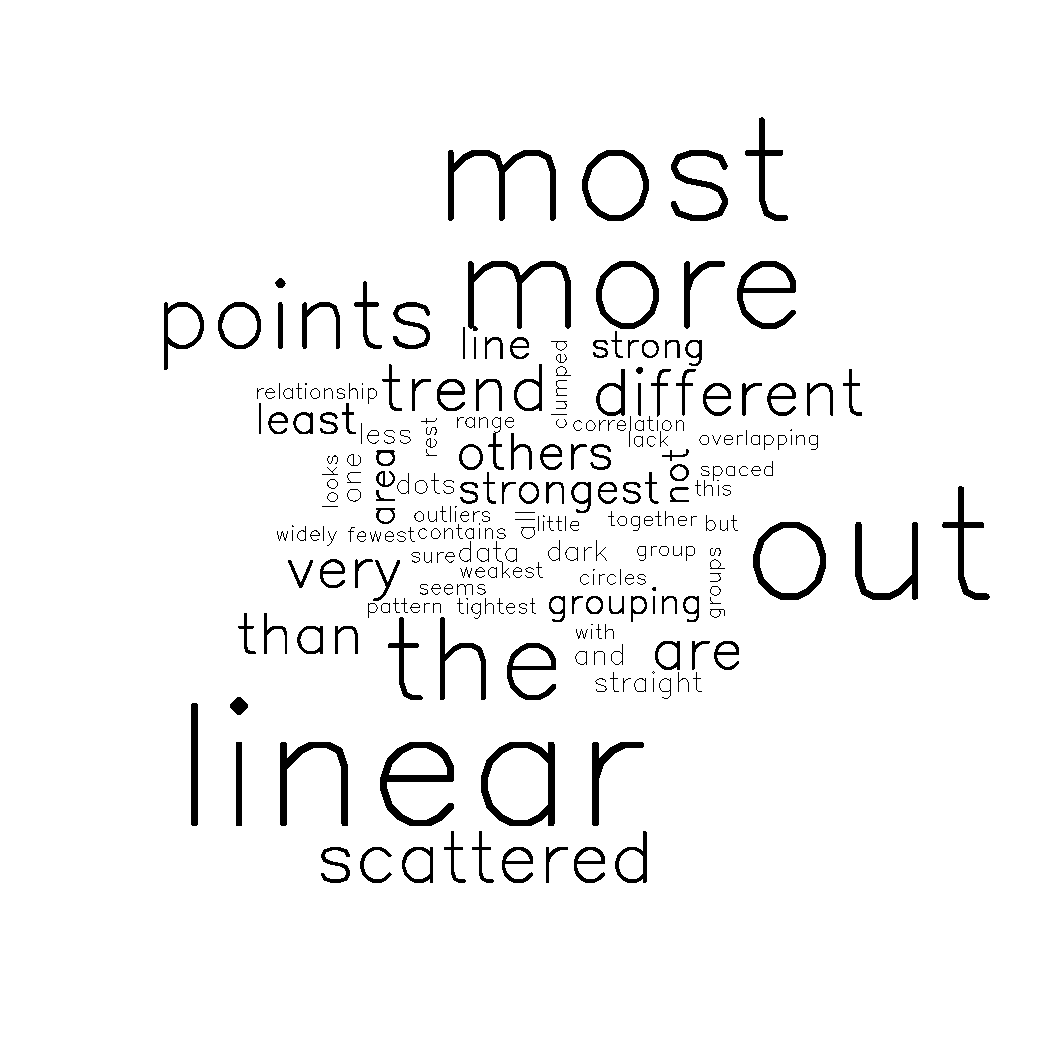
\includegraphics[width=0.9\linewidth]{figure/sentiment-1}
\end{subfigure}
\begin{subfigure}[t]{0.275\linewidth}
  \caption{Plain, cluster target}\vspace{-0.15in}
  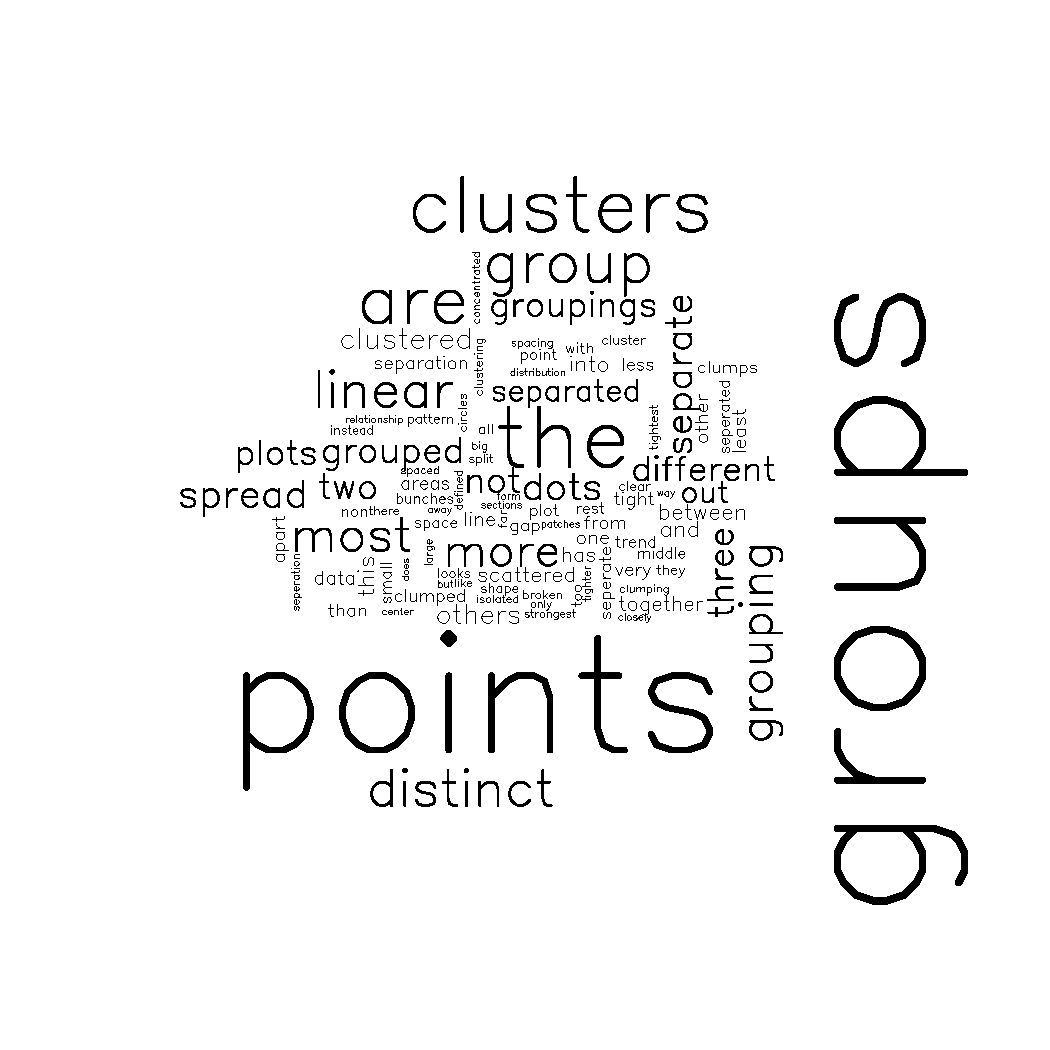
\includegraphics[width=0.9\linewidth]{figure/sentiment-2}
\end{subfigure}
\begin{subfigure}[t]{0.275\linewidth}
  \caption{Plain, trend target}\vspace{-0.15in}
  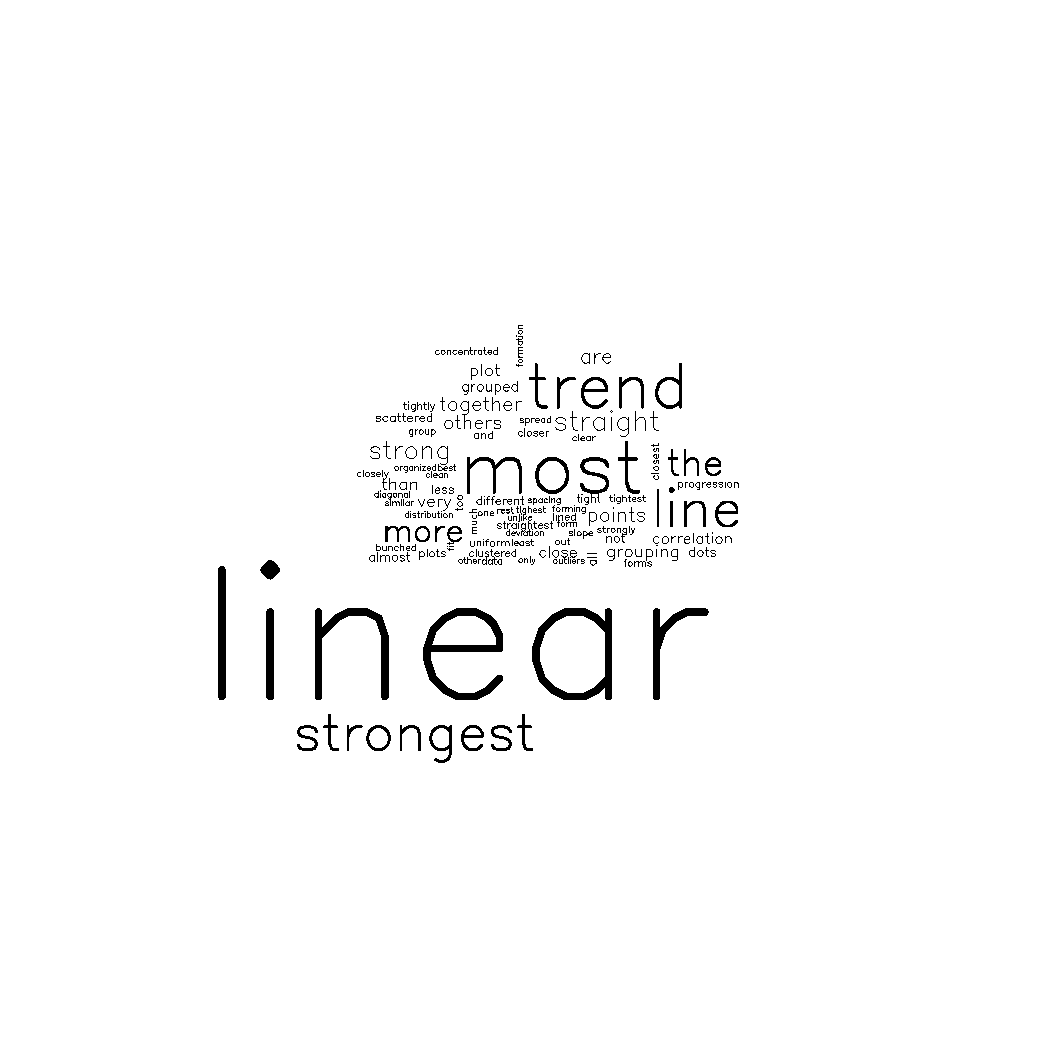
\includegraphics[width=0.9\linewidth]{figure/sentiment-3}
\end{subfigure}

\begin{subfigure}[t]{0.275\linewidth}
  \caption{Trend, neither target}\vspace{-0.2in}
  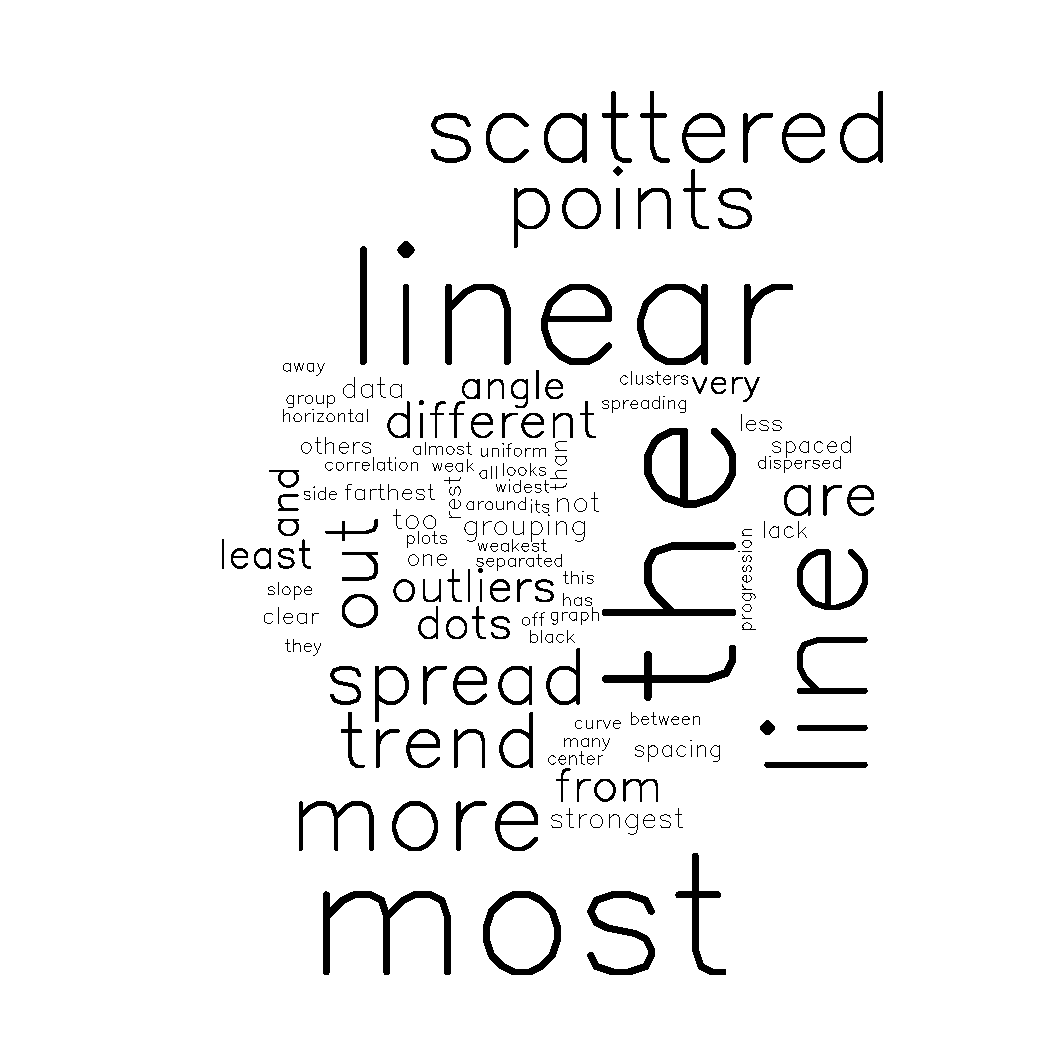
\includegraphics[width=.9\linewidth]{figure/sentiment-4}
\end{subfigure}
\begin{subfigure}[t]{0.275\linewidth}
  \caption{Trend, cluster target}\vspace{-0.2in}
  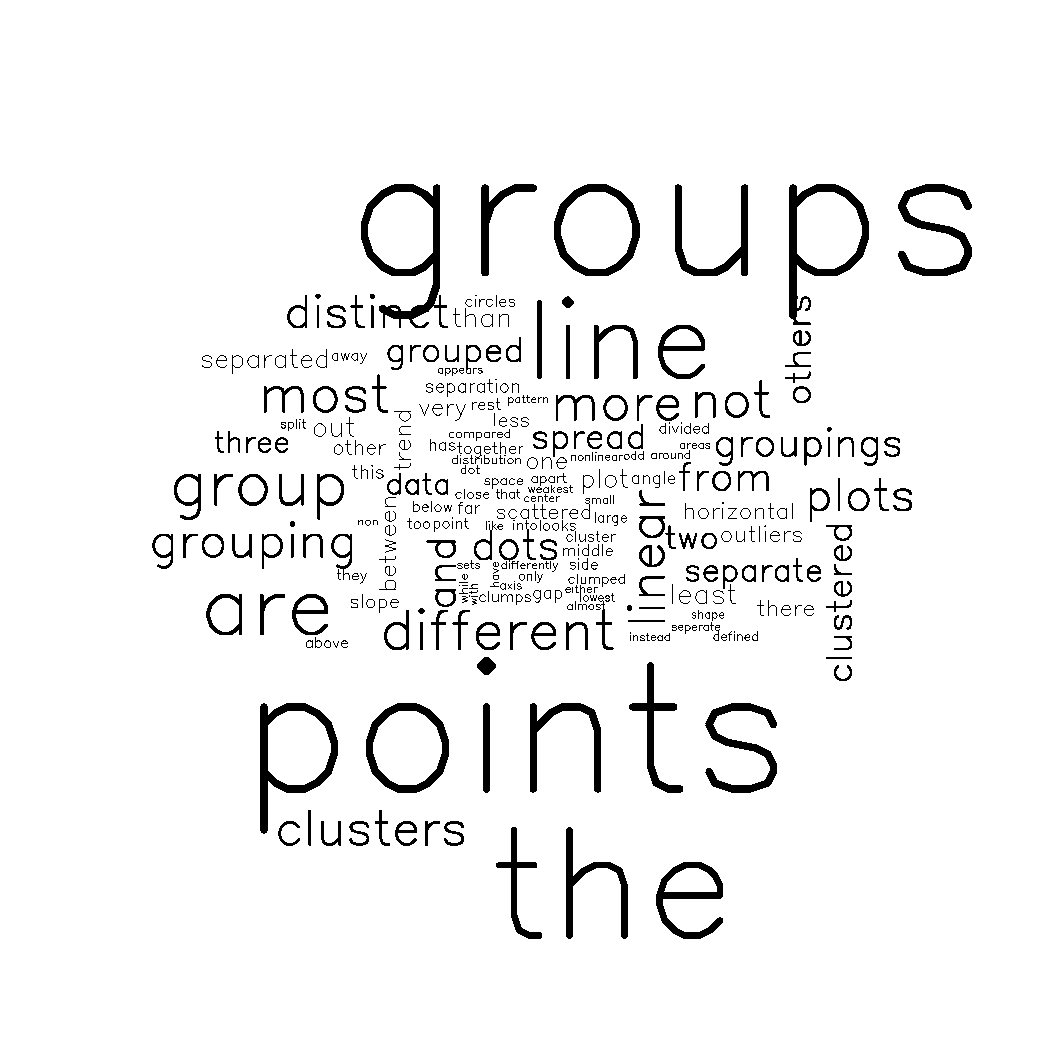
\includegraphics[width=.9\linewidth]{figure/sentiment-5}
\end{subfigure}
\begin{subfigure}[t]{0.275\linewidth}
  \caption{Trend, trend target}\vspace{-0.2in}
  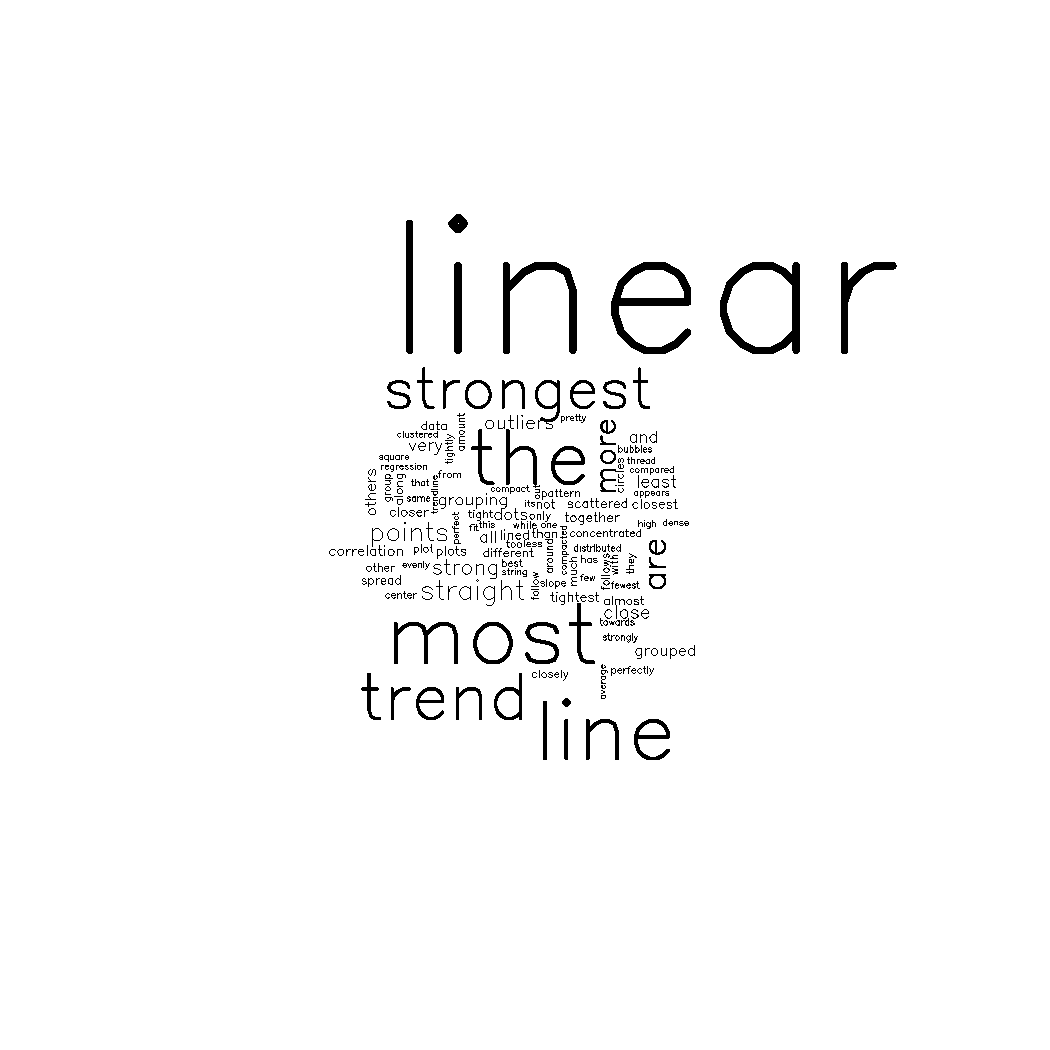
\includegraphics[width=.9\linewidth]{figure/sentiment-6}
\end{subfigure}

\begin{subfigure}[t]{0.275\linewidth}
  \caption{Color, neither target}\vspace{-0.2in}
  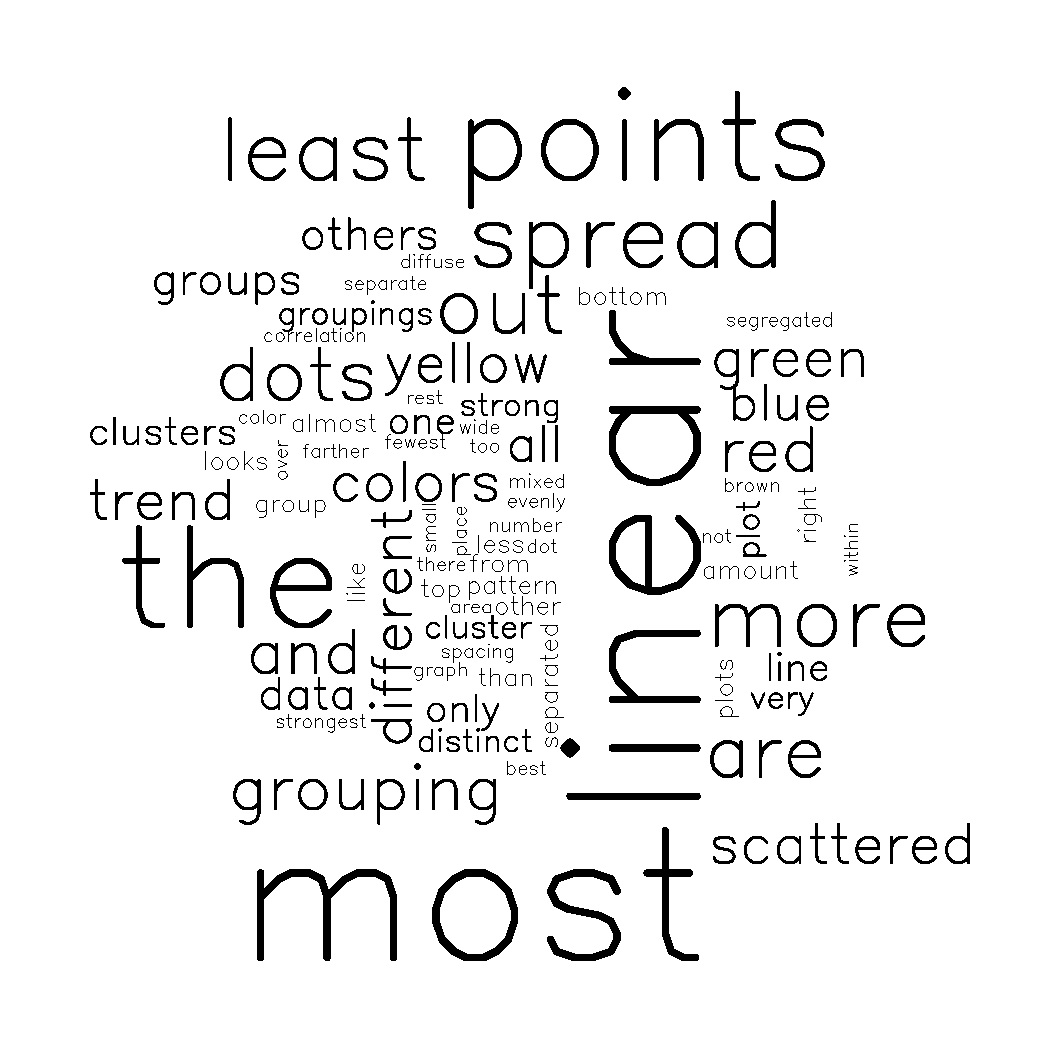
\includegraphics[width=.9\linewidth]{figure/sentiment-7}
\end{subfigure}
\begin{subfigure}[t]{0.275\linewidth}
  \caption{Color, cluster target}\vspace{-0.2in}
  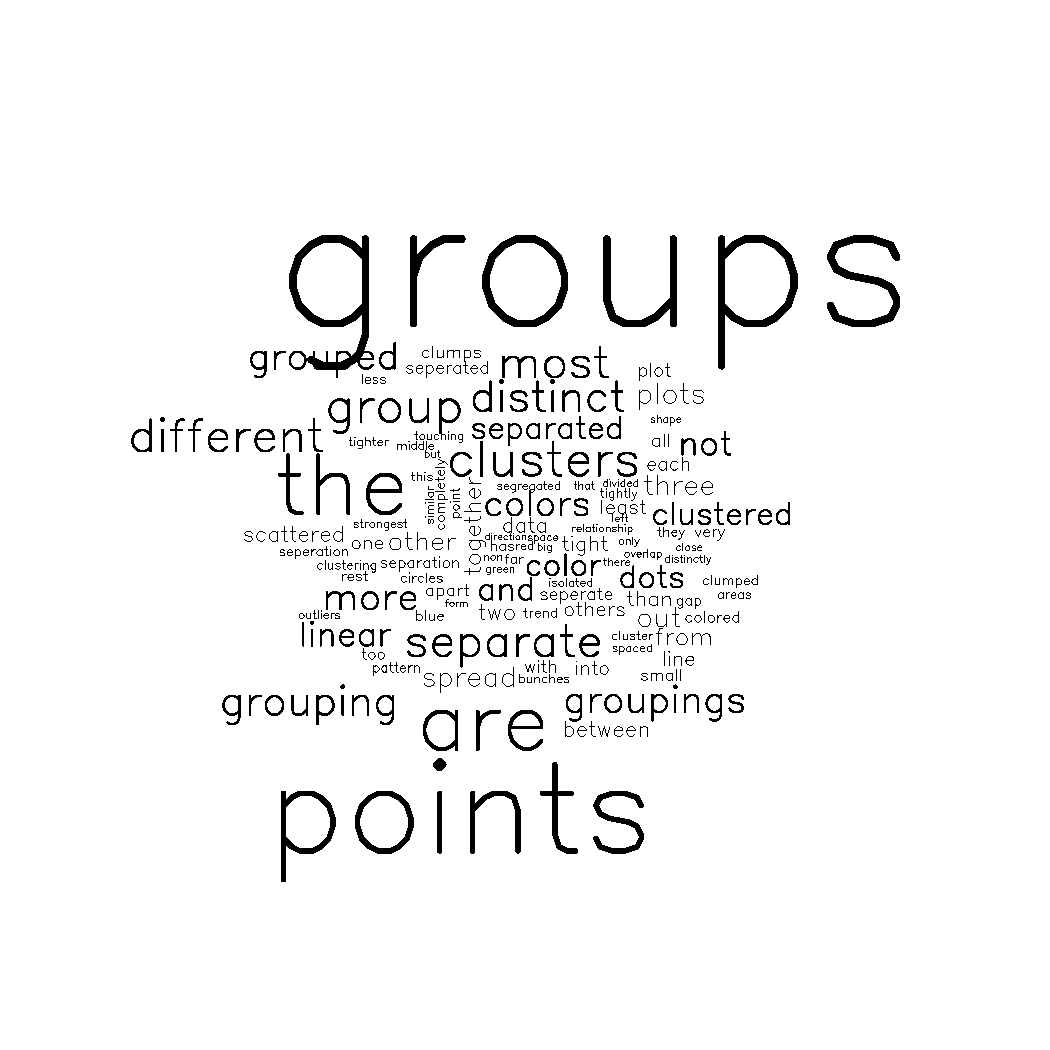
\includegraphics[width=.9\linewidth]{figure/sentiment-8}
\end{subfigure}
\begin{subfigure}[t]{0.275\linewidth}
  \caption{Color, trend target}\vspace{-0.2in}
  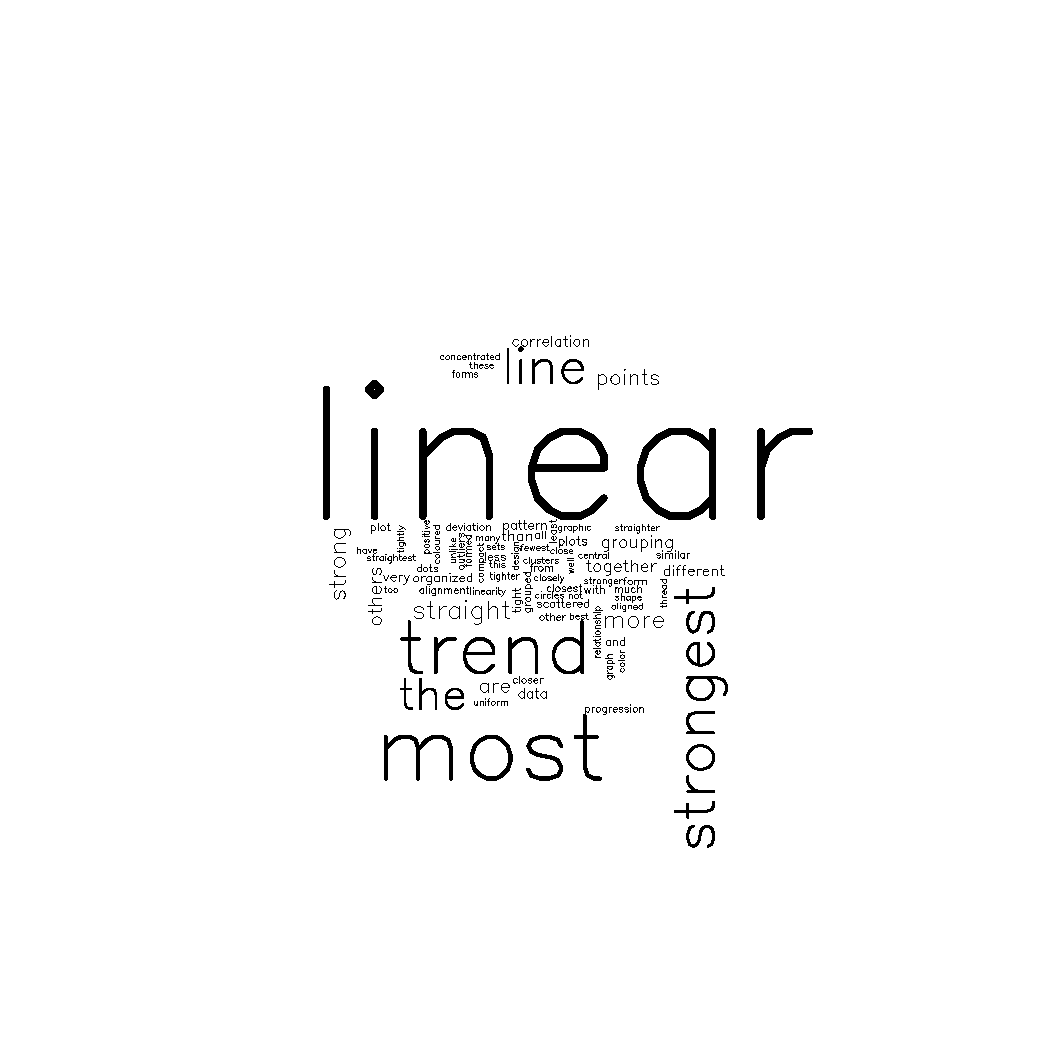
\includegraphics[width=.9\linewidth]{figure/sentiment-9}
\end{subfigure}

\begin{subfigure}[t]{0.275\linewidth}
  \caption{Color + Ellipse, neither}\vspace{-0.2in}
  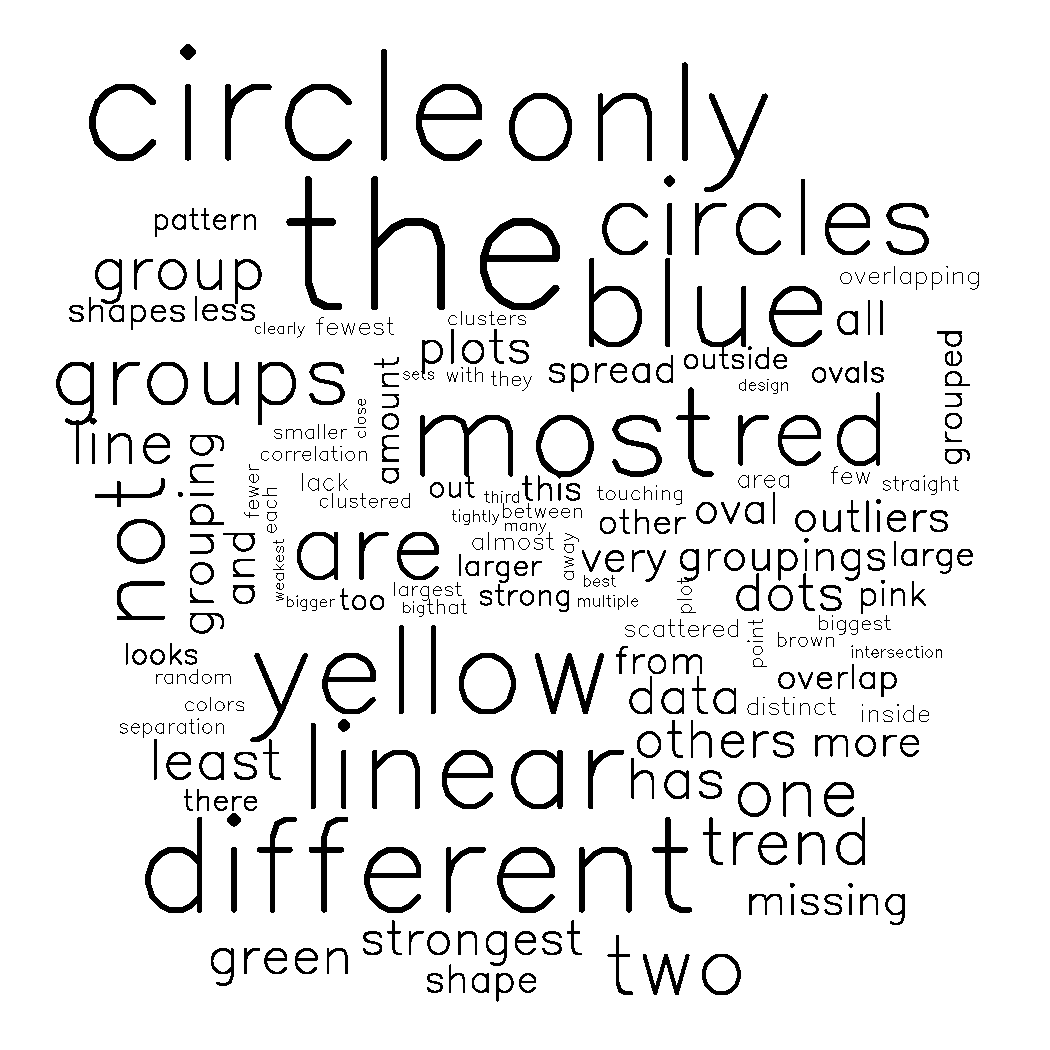
\includegraphics[width=.9\linewidth]{figure/sentiment-10}
\end{subfigure}
\begin{subfigure}[t]{0.275\linewidth}
  \caption{Color + Ellipse, cluster}\vspace{-0.2in}
  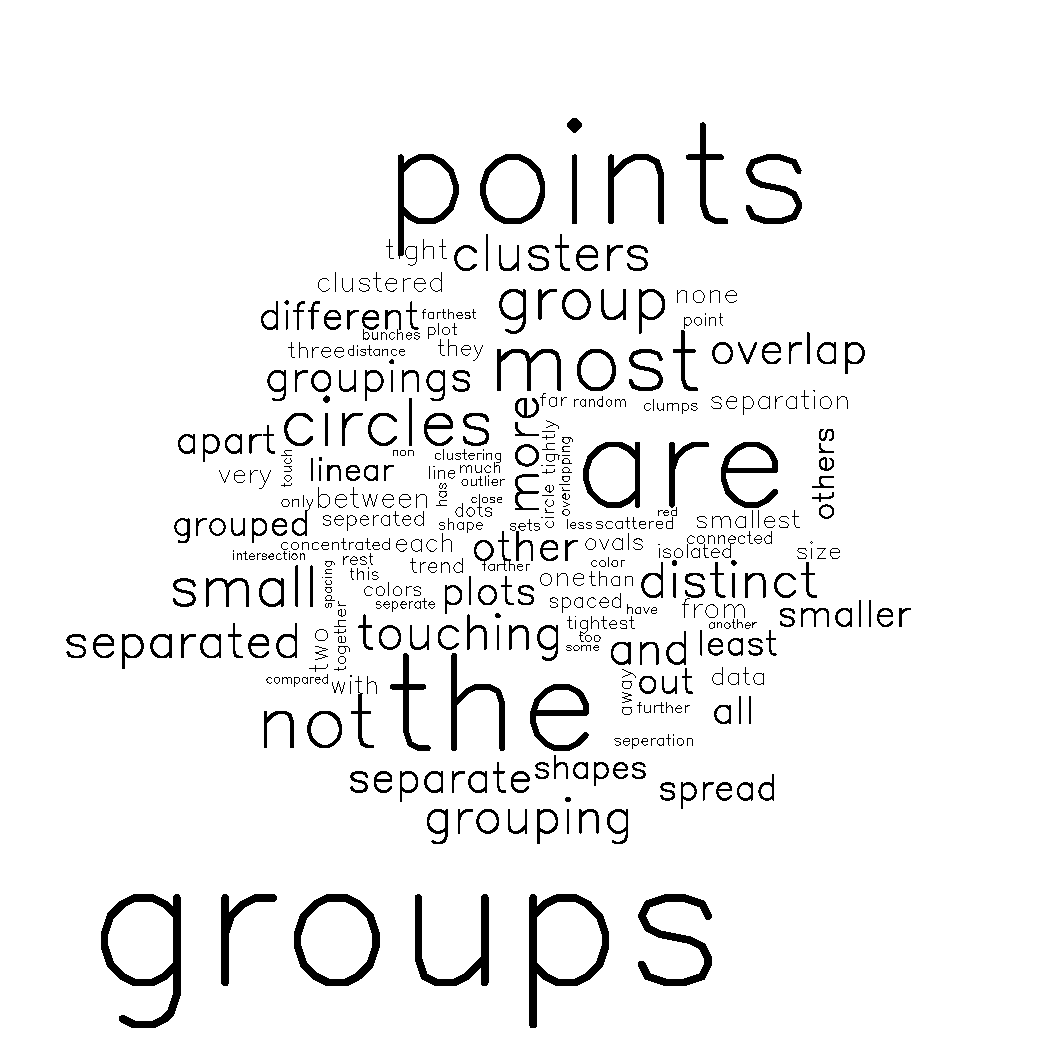
\includegraphics[width=.9\linewidth]{figure/sentiment-11}
\end{subfigure}
\begin{subfigure}[t]{0.275\linewidth}
  \caption{Color + Ellipse, trend}\vspace{-0.2in}
  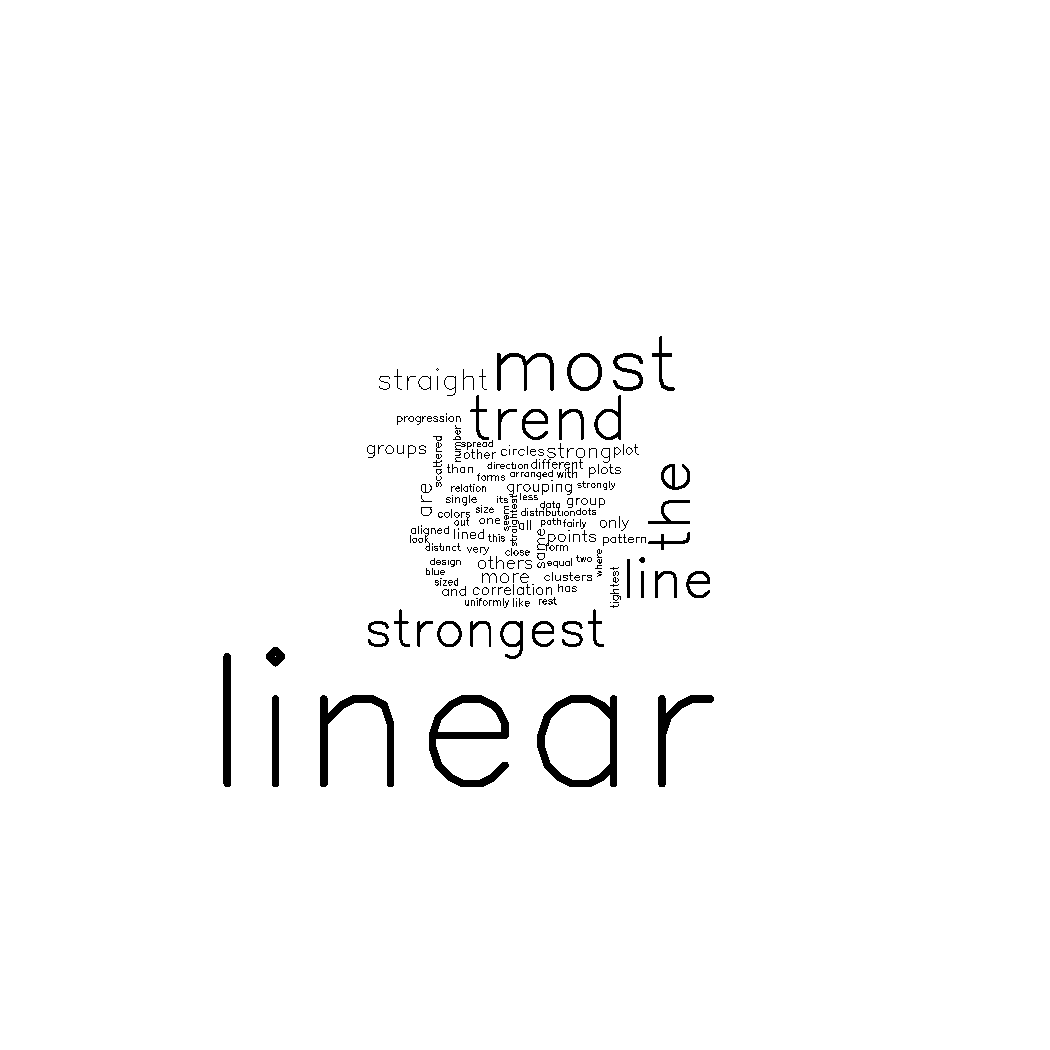
\includegraphics[width=.9\linewidth]{figure/sentiment-12}
\end{subfigure}
\caption[Wordclouds of participant responses for selected plot types]{\label{fig:wordles}Wordclouds of participants' reasoning by outcome for a selected number of plot types. Mostly, the reasoning and the choice of the target are highly associated. For the Color + Ellipse plot, participants were distracted from either target by an imbalance in the cluster/color distribution, as can be seen from the reasoning in the bottom left wordcloud.}
\end{figure}

%' For a more quantitative analysis, responses were categorized based on keywords such as ``line(ar)'', ``correlation'', ``group'', ``cluster'', ``clump'', as well as the presence of negation words (non, not, less, etc.). In addition to linear, nonlinear, and group sentiment, many responses focused on the presence of outliers or the amount of variability present in the chosen plot. 
%' \begin{figure}[ht]\centering
%' <<lexical-analysis, echo=FALSE, fig.width=8, fig.height=6, out.width='.8\\linewidth'>>=
%' lexicaldata <- modeldata
%' lexicaldata$choice_reason <- tolower(lexicaldata$choice_reason)
%' 
%' get.reason <- function(x){
%'   negs <- "non|not|less|weak|least|no|lack|but|divergent"
%'   groups <- "group|cluster|spot|region|separat|clump|space|sets|gap|bunch|apart|connected|segregat|split|overlap|touch|area|tight|intersection|divided"
%'   linear <- "line|linear|correlation|trend|slant|angle|straight|slope"
%'   variability <- "outlier|spread|diffuse|random|scatter"
%'     reasons = data.frame(
%'       linear = str_detect(x, linear) & 
%'         !str_detect(x, negs) &
%'         !str_detect(x, groups),
%'       group = str_detect(x, groups) & 
%'         !str_detect(x, linear),
%'       nonlinear = str_detect(x, linear) & 
%'         str_detect(x, negs) & 
%'         !str_detect(x, groups),
%'       both = str_detect(x, groups) & 
%'         str_detect(x, linear) & 
%'         !str_detect(x, negs),
%'       outliers = str_detect(x, variability) & !str_detect(x, linear) & !str_detect(x, groups)
%'       )
%'     res <- rep("", length(x))
%'     res[rowSums(reasons)==0] <- "other"
%'     if(sum(rowSums(reasons)>1)>1){
%'       warning("Reasons are not mutually exclusive")
%'     }
%'     res[reasons$linear] <- "linear"
%'     res[reasons$nonlinear] <- "nonlinear"
%'     res[reasons$group] <- "group"
%'     res[reasons$both] <- "linear & group"
%'     res[reasons$outlier] <- "outlier"
%'     if(length(res)==1) return(unlist(res))
%'     return(res)
%' }
%' 
%' lexicaldata <- lexicaldata %>% 
%'   mutate(reason = get.reason(choice_reason))
%' 
%' lexicaldata$outcome <- factor(lexicaldata$outcome, levels=c("neither", "trend", "cluster", "both"), labels=c("Neither", "Trend", "Cluster", "Both"))
%' lexicaldata$reason <- factor(lexicaldata$reason, levels=c("group", "nonlinear", "outlier", "linear & group", "linear", "other"), labels=c("Group sentiment", "Non-linear sentiment", "Variability/Outlier sentiment", "Linear + Group sentiment", "Linear sentiment", "Other"))
%' 
%' qplot(data=lexicaldata, x=outcome, fill=reason, geom="histogram", position="dodge") + facet_wrap(~reason) + 
%'   scale_fill_brewer(guide="none", palette="Set1") + 
%'   ylab("# Responses") + 
%'   xlab("Outcome") + 
%'   ggtitle("Sentiment Expressed in Participant Explanations, by Trial Outcome") + 
%'   theme_bw()
%' 
%' @
%' \caption[Lexical analysis of participant reasoning]{Lexical analysis of participants' justification of plot selection. Group sentiment in the reasoning is highly associated with selection of the cluster target plot; linear sentiment is highly associated with selection of the trend target plot.}\label{fig:lexicalanalysis}
%' \end{figure}
%' 
%' \afterpage{\clearpage}
%' The results of this analysis, shown in Figure~\ref{fig:lexicalanalysis} and supported by Figure~\ref{fig:wordles}, indicate that for the most part participants were making decisions based on the criteria we manipulated; rather than alternate visual cues such as group size. In future studies, however, group size should be more tightly controlled to reduce the presence of distractor aesthetics in null plots. 


\section{Discussion and Conclusions}\label{sec:Conclusion}

Taken together, the results presented suggest that plot aesthetics influence the perception of the dominant effect in the displayed data. 
This effect is not simply additive (otherwise, the two conflicting aesthetic conditions would result in similarly neutral effects); rather, the effect is consistent with layering of gestalt perceptual heuristics. 
Plot layers which add additional heuristics show larger effects than plot layers which duplicate heuristics that are already in play. 
For example, adding ellipses to a plot which has color aesthetics increases group recognition by recruiting the common region heuristic in addition to the point similarity heuristic recruited by color. 
Adding shape to a plot which has color aesthetics increases group recognition only slightly, but does not add additional gestalt heuristics (though point similarity is emphasized through two different mechanisms). 

Statistically, this is important because the addition of ellipses or prediction intervals provides important statistical context, while reinforcing the visual emphasis by addition of the common region heuristic. Graphics which more effectively convey the statistical results are composed of aesthetic layers which recruit multiple gestalt heuristics in order to present a unified message. This represents a departure from the ``show the data" mentality, but is still consistent with the goal of good graphics, that is, to convey the data in a way that is easily understandable while still providing appropriate detail. 

While more studies are necessary to fully explore the nonadditive mechanism of additional gestalt heuristics and understand their effect in other types of plots, these results demonstrate the importance of carefully constructing graphs to convey the most important aspects of the displayed data. 

\bibliographystyle{asa}
\bibliography{references}
\newpage
\begin{appendix}
\section{Simulation Studies of Parameter Space}\label{app:parametersimulation}

Using 1000 simulations for each of the 98 combinations of parameters ($K=\{3,5\}$, $\sigma_C=\{.1, .15, .2, .25, .3, .35, .4\}$, $\sigma_T=\{.2, .25, .3, .35, .4, .45, .5\}$), we explored the effect of parameter value on the distribution of summary statistics describing the line strength ($R^2$) and cluster strength for null and target plots. 

Figures~\ref{fig:simulationLineIntervals} and~\ref{fig:simulationClusterIntervals} show the 25th and 75th percentiles of the distribution of $R^2$ and cluster strength summary statistics for each set of parameter values. These plots guide our evaluation of ``easy", ``medium" and ``hard" parameter values for line and cluster tasks. 

Additionally, we note that there is an interaction between $\sigma_C$ and $\sigma_T$: the distinction between target and null on a fixed setting of clustering becomes increasingly difficult as the standard deviation for the linear trend is increased, and vice versa. There may additionally be a three-way interaction between $\sigma_C, \sigma_T$, and $K$: the width of the blue intervals (bottom figure) changes  between different levels of $K$ and for different levels of $\sigma_C$ and $\sigma_T$. These interactions suggest that in order to examine differences in aesthetics, we must block by parameter settings (this can be accomplished through blocking by dataset). Each dataset is non-deterministic, because we have a random process generating from different parameter settings, not a deterministic run setting as in an engineering setting. It is thus important to use replicates of each parameter setting to ensure that we can separate data-level effects from parameter-level effects. 



\begin{figure}[bht]\centering
\begin{subfigure}[t]{.8\linewidth}
\caption{$R^2$ values for target and null data distributions. \label{fig:simulationLineIntervals}}
\vspace{-.15in}
\includegraphics[width=\textwidth]{figure/simulationparameters-1}
\end{subfigure}
\begin{subfigure}[t]{.8\linewidth}
\caption{Cluster cohesion statistics $C^2$. \label{fig:simulationClusterIntervals}}
\vspace{-.15in}
\includegraphics[width=\textwidth]{figure/simulationparameters-2}
\end{subfigure}
\caption{Simulated interquartile ranges between target and most extreme statistic from one of the 18 null plots. }
\end{figure}
\clearpage

\section{Simulation based inference in a two-target lineup scenario}\label{sec:simulation}

Assume that there are two targets embedded in a lineup of overall size $m$, where $m$ in our experiment is taken to be $m=20$. Let $A$ be the event that one of these targets is chosen.
Under the null hypothesis that both targets are consistent with being created based on data from the null model, we can assume that under the null hypothesis the expected value of the probability that an observer picks one of these plots from the lineup is $2/m = E[ P(A \mid H_o) ]$.
For the distribution of $A \mid H_o$ we employ a simulation-based strategy:
Under the null hypothesis, we can assume, that the $p$-value corresponding to a hypothesis test `the presented data is consistent with the null model' has a standard uniform distribution, i.e. $p_i \sim U[0,1]$ i.i.d.~for all $1 \le i \le m$. We assume that the choice observers make can be modeled using a multinomial distribution, where the probability $\pi_i$ to pick panel $i$ is inversely linear to $p_i$, with $\sum_{i=1}^m \pi_i = 1$.

\begin{figure}[h!tbp]

\begin{knitrout}
\definecolor{shadecolor}{rgb}{0.969, 0.969, 0.969}\color{fgcolor}

{\centering \includegraphics[width=0.7\linewidth]{figure/twotarget-1} 

}



\end{knitrout}
\caption{\label{fig:simulation} 
Ten simulations of size $b_2 = 1,000$ and $b_1 = 100$ for lineups of size $m=20$ assuming $K=10$ evaluations. 
The averages of the ten simulation runs are shown as lines. The crosses are probabilities from  Binomial $B_{2/20, 10}$.
}
\end{figure} 

W.l.o.g.\ we can assume that the two target plots are in positions 1 and 2. 
Given that a lineup was evaluated by $K$ individuals, the simulation process for the conditional probability of identifying one of the targets given that both are consistent with the null model, $P(A|H_o)$, is then as follows:
%
\begin{enumerate}
\item Pick two values $p_i \sim U[0,1], i=1, 2$.
\item Repeat $b_1$ times:
\begin{enumerate}
    \item Pick $m-2$ values $p_i \sim U[0,1], i=3, ..., m$.
    \item Pick $K$ values from a Multinomial distribution with $\pi = \frac{1-p}{|| 1- p||}$, i.e. $x_j \sim M_\pi, i=1, ..., K$
    \item Return the number of times that $x_j$ is 1 or 2. 
\end{enumerate} 
\end{enumerate}
Repeat the above process $b_2$ times, and average results for a distribution of $A \mid H_o$. 
The choice of $b_1$ and $b_2$ decides on the number of decimal places to which the estimated distribution can be used reliably. 

Figure~\ref{fig:simulation} shows the result of this simulation approach for a lineup of size 20 assuming $K=10$ evaluation. The density of $A \mid H_o$ is plotted for ten runs (open circles). The variability in the results is relatively small - for comparison, the density of a Binomial distribution $B_{2/20, 10}$ is shown using crosses. The main difference between the densities is the probability of zero or only one identification, while the tail probabilities are very similar.
\end{appendix}
\end{document}
